
\chapter{Rerandomization and Regression Adjustment}
 \label{chapter:rerandomization-regression}


Stratification and post-stratification in Chapter  \ref{chapter::stratification-poststratification} are duals for discrete covariates in the design and analysis of randomized experiments.  How should we deal with multidimensional, possibly continuous, covariates? We can discretize continuous covariates, but this is not an ideal strategy with many covariates. Rerandomization and regression adjustment are duals for general covariates, which are the topics for this chapter. 


The following table summarizes the topics of Chapters  \ref{chapter::stratification-poststratification} and \ref{chapter:rerandomization-regression}:


\begin{center}
\begin{tabular}{c|c|c}
\hline 
 & design & analysis \\ 
 \hline 
 discrete covariate & stratification & post-stratification \\
 \hline 
 general covariate & rerandomization & regression adjustment \\
 \hline 
 \end{tabular}
\end{center}





\section{Rerandomization}

\subsection{Experimental design}
Again we consider a finite population of $n$ experimental units, where $n_1$ of them receive the treatment and $n_0$ of them receive the control. Let
 $\bm{Z} = (Z_1,\ldots, Z_n)$ be the treatment vector for these units. Unit $i$ has covariate $X_i \in \mathbb{R}^K$ which can have continuous or binary components. Concatenate them as an $n\times K$ covariate matrix $\bm{X} = (X_1 , \ldots, X_n )  \tran$ and center them at mean zero $\bar{X}  = n^{-1} \sumn X_i = 0$ to simplify the presentation. 

The CRE balances the covariates in the treatment and control groups on average, for instance, the difference in means of the covariates
$$
\hat{\tau}_X  = n_1^{-1} \sumn Z_i X_i - n_0^{-1} \sumn (1-Z_i) X_i
$$
has mean zero under the CRE. However, it can result in undesired covariate balance across the treatment and control groups in the realized treatment allocation, that is, the realized value of $\hat{\tau}_X  $ is often not zero. Using the vector form of \citet{Neyman:1923} in Problem \ref{hw::vector-neyman1923} before, we can show that
$$
\cov(\hat{\tau}_X  ) 
= \frac{1}{n_1}  S_X^2  + \frac{1}{n_0}  S_X^2   
=  \frac{n}{n_1 n_0} S_X^2   ,
$$
where $ S_X^2   = (n-1)^{-1} \sumn  X_i X_i\tran $ is the finite-population covariance matrix of the covariates. The following Mahalanobis distance measures the difference between the treatment and control groups:
\begin{equation}
\label{eq::m-distance-def}
M = \hat{\tau}_X \tran \cov(\hat{\tau}_X  )^{-1} \hat{\tau}_X  = \hat{\tau}_X \tran  \left(  \frac{n}{n_1 n_0} S_X^2   \right)^{-1} \hat{\tau}_X  . 
\end{equation}
Technically, the above formula for $M$ in \eqref{eq::m-distance-def} is meaningful only if $S_X^2 $ is invertible, which means that the columns of the covariate matrix $\bm{X}$ are linearly independent. If a column can be represented by a linear combination of other columns, it is redundant and should be dropped before the experiment. 
A nice feature of $M$ is that it is invariant under non-degenerate linear transformations of $X$. Lemma \ref{lemma::invariance-mdistance} below summarizes the result with the proof relegated to Problem \ref{para::invariance-M}. 

\begin{lemma}\label{lemma::invariance-mdistance}
$M$ in \eqref{eq::m-distance-def} remains the same if we transform $X_i$ to $b_0  + BX_i$ for all units $i=1,\ldots, n$ where $b_0  \in \mathbb{R}^K$ and $B \in \mathbb{R}^{K\times K}$ is invertible. 
\end{lemma}




The finite population CLT \citep{li2017general} ensures that with large $n$, the Mahalanobis distance $M $ is approximately $ \chi^2_K$ under the CRE. Therefore, it is likely that $M$ has a large realized value under the CRE with asymptotic mean $K$ and variance $2K$. Rerandomization avoids covariate imbalance by discarding the treatment allocations with large values of $M$. Below I give a formal definition of the rerandomization using the Mahalanobis distance (ReM), which was proposed by \citet{cox:1982} and further studied by \citet{morgan2012rerandomization}. 


\begin{definition}
[ReM]
Draw $\bm{Z}$ from CRE and accept it if and only if 
$$
M \leq a,
$$  
for some predetermined constant $a > 0$. 
\end{definition}



The problem of choosing $a$ is similar to the problem of choosing the number of strata in the SRE, which is non-trivial in practice. At one extreme, $a = \infty$, we just conduct the CRE. At the other extreme, $a=0$, there are very few feasible treatment allocations, and consequently, the experiment has little randomness, rendering randomization-based inference useless. As a compromise, we choose a small but not extremely small $a$, for example, $a=0.001$ or some upper quantile of a $\chi^2_K$ distribution. 


 

ReM has many desirable properties. As mentioned above, it is invariant to linear transformations of the covariates. Moreover, it has nice geometric properties and elegant mathematical theory. This chapter will focus on ReM.  


\subsection{Statistical inference}

An important question is how to analyze the data under ReM. \citet{bruhn2009pursuit} and \citet{morgan2012rerandomization} argued that we can always use the FRT as long as we simulate $\bm{Z}$ under the constraint $M\leq a$. This always yields finite-sample exact $p$-values under the sharp null hypothesis. See Problem \ref{hw::FRT-under-REM}. 


It is a challenging problem to derive the finite sample properties of ReM without assuming the sharp null hypothesis. Instead, \citet{li2018asymptotic} derived the asymptotic distribution of the difference in means of the outcome $\hat{\tau}$ under ReM and the regularity conditions below.



\begin{condition}\label{condition::regularity-cre-rem}
As $n\rightarrow \infty$,
\begin{enumerate}
\item 
$n_1/n$ and $n_0/n$ have positive limits;
\item 
the finite population covariance of $\{  X_i, Y_i(1), Y_i(0), \tau_i \}$ has a finite limit;
\item
$\max_{1\leq i \leq n}  \{   Y_i(1) - \bar{Y}(1) \} ^2/n \rightarrow 0 $,
$\max_{1\leq i \leq n}  \{   Y_i(0) - \bar{Y}(0) \}^2/n \rightarrow 0 $,
and $\max_{1\leq i \leq n}   X_i \tran X_i/n \rightarrow 0 $,
\end{enumerate}
\end{condition} 


Below is the main theorem for ReM, which relies on additional notation.    
Let 
$$
L_{K,a} \sim D_1\mid \bm{D}\tran \bm{D} \leq a
$$ 
where $\bm{D} = (D_1,\ldots, D_K)$ follows a $K$-dimensional standard Normal distribution; let $ \varepsilon$ follow a univariate standard Normal distribution; $L_{K,a}  \ind \varepsilon .$


\begin{theorem}\label{thm::remasymptotics}
Under ReM with $M\leq a$ and Condition \ref{condition::regularity-cre-rem}, we have\footnote{The notation ``$A \asim B$'' means that $A$ and $B$ have the same asymptotic distributions.} 
$$
\hat{\tau} - \tau \asim \sqrt{ \var(\hat \tau) }  \left\{   \sqrt{R^2} L_{K,a}  + \sqrt{1-R^2} \varepsilon \right\},
$$
where 
$$
\var( \hat{\tau} ) = \frac{S^2(1)}{n_1} + \frac{S^2(0)}{n_0} - \frac{S^2(\tau)}{n}
$$
is \citet{Neyman:1923}'s variance formula proved in Chapter \ref{chapter::neyman-cr}, and
$$
R^2 = \textup{corr}^2(\hat{\tau}, \hat{\tau}_X   )
$$
is the squared multiple correlation coefficient (see Section \ref{sec::measure-pearson-r2} for the definition)  between $\hat{\tau}$ and $\hat{\tau}_X $ under the CRE.
\end{theorem}


Although the proof of \citet{li2018asymptotic} is technical, the asymptotic distribution in Theorem \ref{thm::remasymptotics} has a clear geometric interpretation, as shown in Figure \ref{fig::geometry-rem}. It shows that $\hat\tau$ decomposes into a component that is a linear combination of $\hat\tau_X$ and a component that is orthogonal to $\hat\tau_X$. Geometrically, $\cos^2 \theta = R^2$, where $\theta$ is the angle between $\hat\tau$ and $\hat\tau_X$.
ReM affects the first component but does not change the second component. The truncated Normal distribution $L_{K,a}$ is due to the restriction of ReM on the first component.  


\begin{figure}
\centering
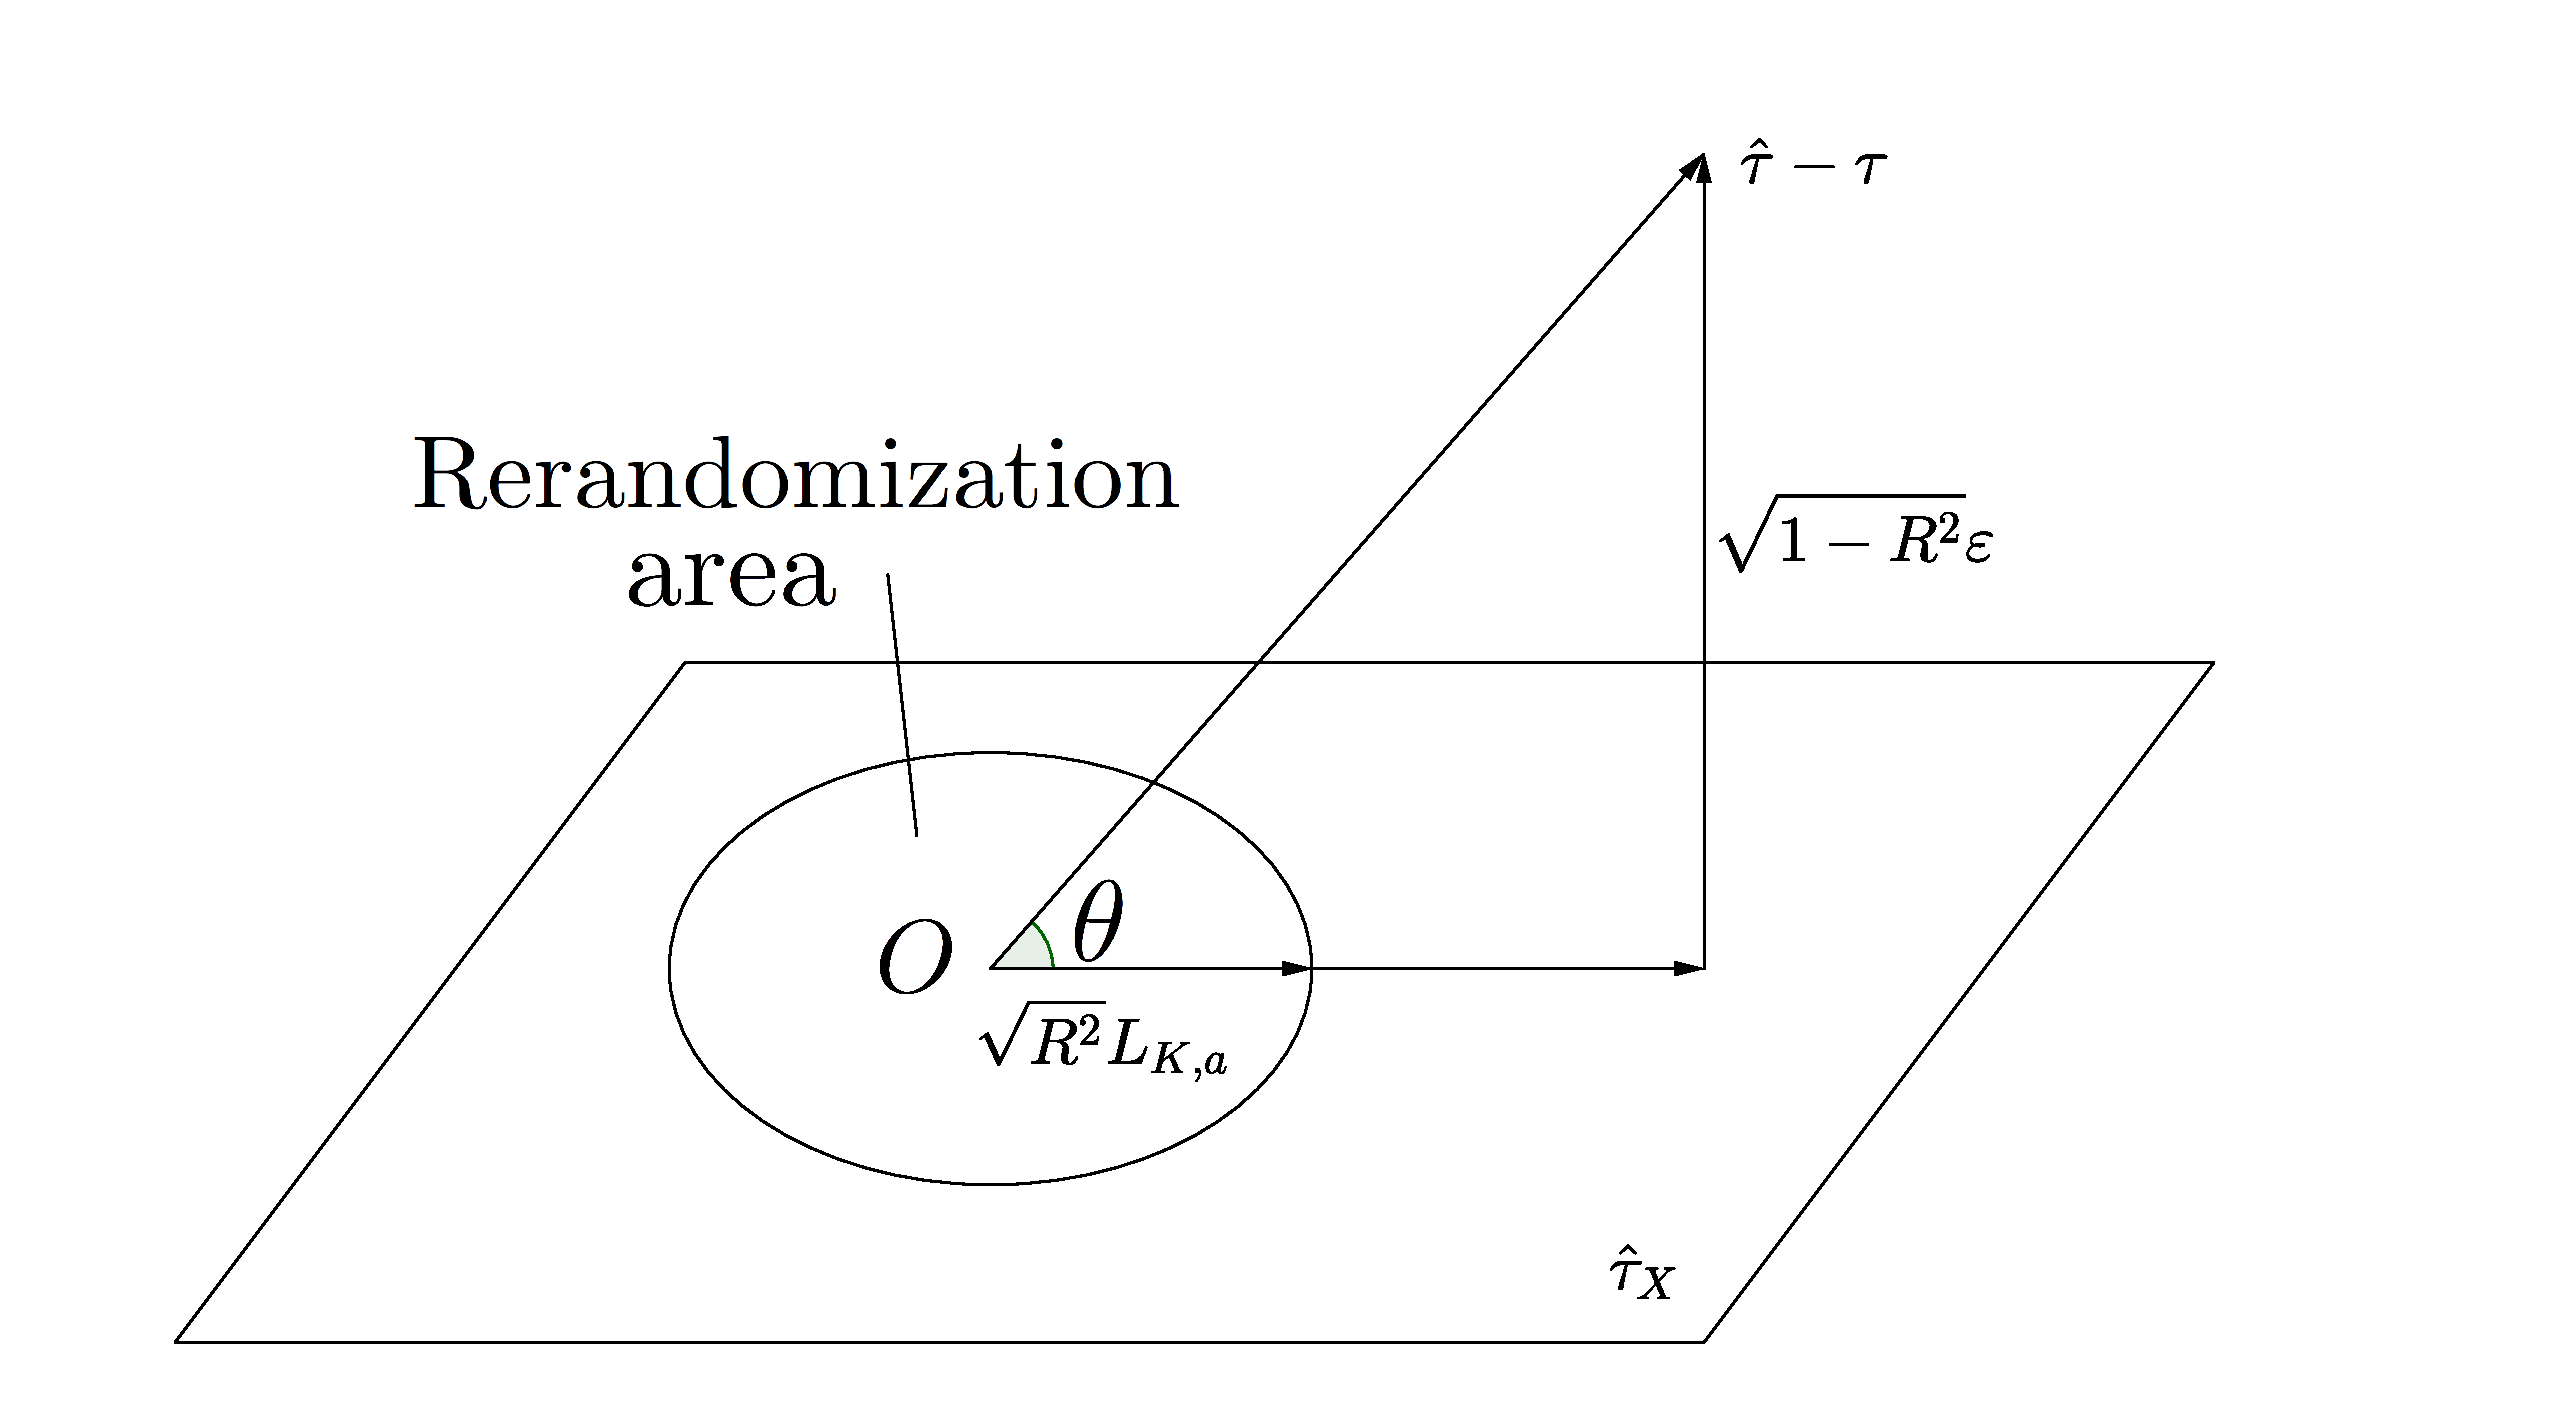
\includegraphics[width = 0.9\textwidth]{figures/rem_geometry.pdf}
\caption{Geometry of the asymptotic distribution of $\hat\tau$  under  ReM}\label{fig::geometry-rem}
\end{figure}


When $a  = \infty$, the asymptotic distribution  simplifies to the one under the CRE:
$$
\hat{\tau} - \tau \asim \sqrt{ \var(\hat \tau) } \varepsilon .
$$
When the threshold $a$ is close to zero, the asymptotic distribution  simplifies to
$$
\hat{\tau} - \tau \asim \sqrt{ \var(\hat \tau) (1-R^2)} \varepsilon ;
$$
see \citet{wang2022rerandomization} for a rigorous proof.
So with a small threshold $a$, the efficiency gain due to ReM depends on $R^2$, which has the following equivalent form. 
\begin{proposition}
\label{prop::rsquared-forms}
Under the CRE, we have 
$$
R^2 = \textup{corr}^2(\hat{\tau}, \hat{\tau}_X   )
= \frac{  n_1^{-1}  S^2(1\mid X) + n_0^{-1} S^2(0\mid X) - n^{-1} S^2(\tau \mid X) }
{ n_1^{-1}  S^2( 1 ) + n_0^{-1} S^2( 0 ) - n^{-1} S^2( \tau  )},
$$
where $\{S^2( 1 ) , S^2( 0 ), S^2( \tau  )\}$ are the finite population variances of $\{ Y_i(1), Y_i(0), \tau_i \}_{i=1}^n$, and $\{S^2( 1 \mid x ) , S^2( 0 \mid x ), S^2( \tau  \mid x )\}$ are the corresponding finite population variances of their linear projections on $(1, X_i)$; see Section \ref{sec::sampleOLS} for the definition of linear projections. 
%\footnote{For example, the linear projection of $Y_i(1)$ on $(1,X_i)$ is $\alpha_1 + \beta_1 X_i$ where 
%$$
%(\alpha_1, \beta_1) = \arg \min_{a,b} \sumn \{  Y_i(1) - a - b\tran X_i\}^2.
%$$
%}
Under the constant causal effect assumption with $\tau_i = \tau$, the $R^2 $ reduces to $S^2(0\mid X) / S^2( 0 ) $, the finite population squared multiple correlation between $Y_i(0)$ and $X_i$.
\end{proposition}

I leave the proof of Proposition \ref{prop::rsquared-forms} to Problem \ref{para::r2-cre}. 

When $ 0 < a <\infty$, the asymptotic distribution of $\hat{\tau}$ has a more complicated form and is more concentrated at $\tau$ and thus the difference in means $\hat{\tau}$ is more precise under ReM than under the CRE. 


If we ignore the design of ReM and still use the confidence interval based on \cite{Neyman:1923}'s variance formula and the Normal approximation, it is overly conservative and overcovers $\tau$ even if the individual causal effects are constant. \citet{li2018asymptotic} proposed to construct confidence intervals based on Theorem \ref{thm::remasymptotics}. We omit the discussion here but will come back to the inference issue in Section \ref{sec::unification-rem-regadj}. 
 



\section{Regression adjustment}

What if we do not conduct rerandomization in the design stage but want to adjust for covariate imbalance in the analysis stage of the CRE? We will discuss several regression adjustment strategies. 

\subsection{Covariate-adjusted FRT}\label{sec::covariate-adjusted-frt-intro}


The covariates $\bm{X}$ are all fixed, and furthermore, under $\HF$, the observed outcomes are all fixed. Therefore, we can simulate the distribution of any test statistic $T = T(\bm{Z}, \bm{Y}, \bm{X})$ and calculate the $p$-value. The basic idea of the FRT remains the same in the presence of additional covariates.  


There are two general strategies to construct the test statistic. Problem \ref{hw::frt-covariates} before hints at both of them. I summarize them below, using the terminology from \citet{zhao2020caFRT}. 


\begin{definition}
[pseudo-outcome strategy for covariate-adjusted FRT]
\label{def::pseudo-y-frt}
We can construct the test statistic based on residuals from fitted statistical models. We can regress $Y_i$ on $X_i$ to obtain residual $\hat \varepsilon_i$, and then treat $\hat \varepsilon_i$ as the pseudo outcome to construct test statistics.
\end{definition}



\begin{definition}
[model-output strategy for covariate-adjusted FRT]
\label{def::model-out-frt}
We can use a regression coefficient as a test statistic. We can regress  $Y_i$ on $(Z_i, X_i)$ to obtain the coefficient of $Z_i$ as the test statistic.
\end{definition}

 

In the pseudo-outcome strategy in Definition \ref{def::pseudo-y-frt}, the regression of $Y_i$ on $X_i$ should not include the treatment $Z_i$ because we want to ensure that the pseudo outcome satisfies $\HF$ if the original outcome satisfies $\HF$. 
In the model-output strategy in Definition \ref{def::model-out-frt}, the regression of $Y_i$ on $(Z_i, X_i)$ includes the treatment $Z_i$ because we want to use the coefficient of $Z_i$ to measure the deviation from $\HF$.  
Computationally, in strategy one, we only need to run regression once, whereas in strategy two, we need to run regression many times. 

In the above,  ``regression'' is a generic term, which can be linear regression, logistic regression, or even machine learning algorithms. The FRT with any test statistics from these two strategies will be finite-sample exact under $\HF$ although they differ under alternative hypotheses. 
The rest of this section will review some test statistics based on OLS. 



\subsection{Analysis of covariance and extensions}\label{sec::ancova}

Now we turn to direct estimation of the average causal effect $\tau$ that adjusts for the observed covariates. 

Historically, \citet{fisher1925statistical} proposed to use the analysis of covariance (ANCOVA) to improve estimation efficiency. This remains a standard strategy in many fields. He suggested running the OLS of $Y_i$ on $(1, Z_i, X_i)$ and obtaining the coefficient of $Z_i$ as an estimator for $\tau$. Let $\hat{\tau}_\textsc{F}$ denote Fisher's ANCOVA estimator. 


A former Berkeley Statistics Professor, David A. Freedman, reanalyzed Fisher's ANCOVA under \citet{Neyman:1923}'s potential outcomes framework. \citet{freedman2008regression_a, freedman2008regression_b} found the following negative results:
\begin{enumerate}
[(1)]
\item
$\hat{\tau}_\textsc{F}$ is biased, but the simple difference in means $\hat{\tau}$ is unbiased.
\item 
The asymptotic variance of $\hat{\tau}_\textsc{F}$ may be even larger than that of $\hat{\tau}$ when $n_1\neq n_0$.
\item 
The standard error from the OLS is inconsistent for the true standard error of $\hat{\tau}_\textsc{F}$ under the CRE.   
\end{enumerate}


A former Berkeley Ph.D. student, Winston Lin, wrote a thesis in response to Freedman's critiques. \citet{lin2013} found the following positive results:
\begin{enumerate}
[(1)]
\item
The bias of $\hat{\tau}_\textsc{F}$ is small in large samples, and it goes to zero as the sample size approaches infinity.
\item
We can improve the asymptotic efficiency of both $\hat{\tau}$ and $\hat{\tau}_\textsc{F}$ by using the coefficient of $Z_i$ in the OLS of $Y_i$ on $(1, Z_i, X_i, Z_i\times X_i)$. Let $\hat{\tau}_\textsc{L}$ denote \citet{lin2013}'s estimator. Moreover, the EHW standard error is a conservative estimator for the true standard error of $\hat{\tau}_\textsc{L}$ under the CRE. 
\item
The EHW standard error\footnote{Without covariates, the HC2 correction yields identical variance estimator as \citet{Neyman:1923}'s classic one; see Problem \ref{hw::neyman-ols-nox}. For coherence, we can also use the HC2 correction for \citet{lin2013}'s estimator with covariate adjustment. When the number of covariates is small compared with the sample size and the covariates do not contain outliers, the variants of the EHW standard error perform similarly to the original one. When the number of covariates is large compared with the sample size or the covariates contain outliers, the variants can outperform the original one. In those cases, \citet{lei2018regression} recommend using the HC3 variant of the EHW standard error.} 
for $\hat{\tau}_\textsc{F}$ in the OLS fit of $Y_i$ on $(1, Z_i, X_i)$ is  a conservative estimator for the true standard error of $\hat{\tau}_\textsc{F}$ under the CRE. 
\end{enumerate}


\subsubsection{Some heuristics for \citet{lin2013}'s results}


\citet{Neyman:1923}'s result demonstrates that the variance of the difference-in-means estimator $\hat{\tau}$ depends on the variances of the potential outcomes. Intuitively, we can reduce the variance of the estimator by reducing the variances of the potential outcomes. A family of linearly adjusted estimators is
\begin{eqnarray} 
\hat{\tau}(\beta_1, \beta_0) &=& n_1^{-1} \sumn Z_i(Y_i - \beta_1\tran X_i) - n_0^{-1} \sumn (1-Z_i) (Y_i - \beta_0\tran X_i)  \label{eq::linear-adj-1}\\
&=& \left\{  \hat{\bar{Y}}(1) - \beta_1\tran \hat{\bar{X} }(1) \right\}  -  \left\{   \hat{\bar{Y}}(0) - \beta_0\tran \hat{\bar{X} }(0) \right\},
\label{eq::linear-adj-2}
\end{eqnarray}
where $\{ \hat{\bar{Y}}(1), \hat{\bar{Y}}(0) \}$ are the sample means of the outcomes, and $\{ \hat{\bar{X} }(1), \hat{\bar{X} }(0)\}$ are the sample means of the covariates. This covariate-adjusted estimator $\hat{\tau}(\beta_1, \beta_0)$ tries to reduce the variance of $\hat\tau$ by residualizing the potential outcomes. It reduces to $\hat\tau$ with $\beta_1 = \beta_0 = 0$. 
It has mean $\tau$ for any fixed values of $\beta_1$ and $\beta_0$ because $\bar{X}  = 0.$ We are interested in finding the $(\beta_1, \beta_0)$ that minimize the variance of $\hat{\tau}(\beta_1, \beta_0)$. This estimator is essentially the difference in means of the adjusted potential outcomes $\{ Y_i(1) - \beta_1\tran X_i  , Y_i(0) - \beta_0\tran  X_i \}_{i=1}^n $. Applying \citet{Neyman:1923}'s result, this estimator has variance
$$
\var\{ \hat{\tau}(\beta_1, \beta_0) \} = \frac{ {S}^2(1; \beta_1) }{ n_1 } + \frac{ {S}^2(0; \beta_0) }{ n_0 }
- \frac{  S^2(\tau; \beta_1, \beta_0)  }{ n },
$$
where $ {S}^2(z; \beta_z)$ $(z=1,0)$ and $S^2(\tau; \beta_1, \beta_0)$ are the finite population variances of the adjusted potential outcomes and individual causal effects, respectively; moreover,  a conservative variance estimate is 
$$
\hat{V}( \beta_1, \beta_0 ) = \frac{ \hat{S}^2(1; \beta_1) }{ n_1 } + \frac{ \hat{S}^2(0; \beta_0) }{ n_0 },
$$
where 
\begin{eqnarray*}
\hat{S}^2(1; \beta_1) &=& (n_1-1)^{-1} \sumn Z_i  ( Y_i - \gamma_1 - \beta_1\tran  X_i )^2,\\ 
\hat{S}^2(0; \beta_0) &=& (n_0-1)^{-1} \sumn (1-Z_i)  ( Y_i - \gamma_0 - \beta_0\tran  X_i )^2
\end{eqnarray*}
are the sample variances of the adjusted potential outcomes with $\gamma_1$ and $\gamma_0$ being the sample means of  $Y_i - \beta_1\tran  X_i$ under treatment and $Y_i   - \beta_0\tran  X_i $ under control. 
To minimize $\hat{V}( \beta_1, \beta_0 )$, we need to solve two OLS problems\footnote{
We can also minimize the true variance of $\hat{\tau}(\beta_1, \beta_0) $. 
See Problem \ref{hw::compare-true-variance} for more details. 
}:
$$
\min_{\gamma_1 , \beta_1 }
\sumn Z_i  ( Y_i - \gamma_1 - \beta_1\tran  X_i )^2,\quad
\min_{\gamma_0 , \beta_0 }
\sumn (1-Z_i)  ( Y_i - \gamma_0 - \beta_0\tran  X_i  )^2.
$$
We run OLS of $Y_i$ on $X_i$ for the treatment and control groups separately and obtain $( \hat{\gamma}_1, \hat{\beta}_1 )$ and $( \hat{\gamma}_0, \hat{\beta}_0 )$. The final estimator is
\begin{eqnarray*}
 \hat{\tau}( \hat{\beta}_1, \hat{\beta}_0) &=& n_1^{-1} \sumn Z_i(Y_i - \hat{\beta}_1\tran  X_i) 
- n_0^{-1} \sumn (1-Z_i)  (Y_i - \hat{\beta}_0\tran  X_i) \\
&=&\left\{  \hat{\bar{Y}}(1) - \hat \beta_1\tran \hat{\bar{X} }(1) \right\}  
-  \left\{   \hat{\bar{Y}}(0) - \hat \beta_0\tran \hat{\bar{X} }(0) \right\} . 
\end{eqnarray*}
From the properties of the OLS fits (see \eqref{eq::OLS-mean-data}), we know
$$
\hat{\bar{Y}}(1) =  \hat{\gamma}_1 + \hat{\beta}_1\tran  \hat{\bar{X} }(1),\quad
\hat{\bar{Y}}(0) =  \hat{\gamma}_0 + \hat{\beta}_0\tran  \hat{\bar{X} }(0).
$$
Therefore, we can rewrite the estimator as
\begin{equation}
\label{eq::lin-intercepts}
 \hat{\tau}( \hat{\beta}_1, \hat{\beta}_0)  =  \hat{\gamma}_1 - \hat{\gamma}_0  
\end{equation}
The equivalent form in \eqref{eq::lin-intercepts} suggests that we can obtain $ \hat{\tau}( \hat{\beta}_1, \hat{\beta}_0) $ from a single OLS fit below.




\begin{proposition}\label{prop::lin-ols}
The estimator $ \hat{\tau}( \hat{\beta}_1, \hat{\beta}_0) $ in \eqref{eq::lin-intercepts} equals the coefficient of $Z_i$ in the OLS fit of $Y_i$ on $(1, Z_i, X_i, Z_i\times X_i)$, which is \citet{lin2013}'s estimator $\hat{\tau}_\textsc{L}$ introduced before. 
\end{proposition}

I leave the proof of Proposition \ref{prop::lin-ols} to Problem \ref{para::lin-ols-covadj}, which is a pure linear algebra fact. 


Based on the discussion above, a conservative variance estimator for $\hat{\tau}_\textsc{L}$ is 
\begin{eqnarray*}
\hat{V}(  \hat{\beta}_1, \hat{\beta}_0 ) 
%= \frac{ \hat{S}^2(1; \hat{\beta}_1) }{ n_1 } + \frac{ \hat{S}^2(0; \hat{\beta}_0) }{ n_0 }
&=& \frac{1}{n_1(n_1 - 1)} \sumn Z_i  ( Y_i - \hat{\gamma}_1 - \hat{\beta}_1\tran  X_i  ) ^2 \\
&& \qquad + \frac{1}{n_0(n_0 - 1)} \sumn (1-Z_i)  ( Y_i - \hat{\gamma}_0 - \hat{\beta}_0\tran  X_i )^2.
\end{eqnarray*}
Based on quite technical calculations, \citet{lin2013} further showed that the EHW standard error from the OLS in Proposition \ref{prop::lin-ols} is almost identical to $\hat{V}(  \hat{\beta}_1, \hat{\beta}_0 ) $ which is a conservative estimator of the true standard error of $\hat{\tau}_\textsc{L}$ under the CRE. Intuitively, this is because we do not assume that the linear model is correctly specified, and the EHW standard error is robust to model misspecification. 



There is a subtle issue with the discussion above. The variance formula $\var\{ \hat{\tau}(\beta_1, \beta_0) \} $ works for fixed $(\beta_1, \beta_0)$, but the estimator $ \hat{\tau}( \hat{\beta}_1, \hat{\beta}_0) $ uses two estimated coefficients $( \hat{\beta}_1, \hat{\beta}_0) $. The additional uncertainty in the estimated coefficients may cause finite-sample bias in the final estimator. \citet{lin2013} showed that this issue goes away asymptotically because $ \hat{\tau}( \hat{\beta}_1, \hat{\beta}_0) $ behaves similarly to $ \hat{\tau}( \tilde{\beta}_1, \tilde{\beta}_0) $, where $\tilde{\beta}_1$ and $\tilde{\beta}_0$ are the limit of $\hat{\beta}_1$ and $ \hat{\beta}_0$, respectively. Heuristically, the difference between  $ \hat{\tau}( \hat{\beta}_1, \hat{\beta}_0) $ and $ \hat{\tau}( \tilde{\beta}_1, \tilde{\beta}_0) $ depends on 
$$
(\hat{\beta}_z - \tilde{\beta}_z)\tran \hat{\bar{X} }(z) ,\quad (z=0,1) 
$$
which is a product of two terms of small order. As a warning,  the asymptotic theory requires a large sample size and some regularity conditions on the potential outcomes and covariates. In finite samples, regression adjustment can be even harmful due to the additional uncertainty in the estimated coefficients $\hat{\beta}_1$ and $\hat{\beta}_0$. 




\subsubsection{Understanding \citet{lin2013}'s estimator via predicting the potential outcomes}
\label{sec::understand-lin-predict}
 
\begin{table}
\centering
\caption{Predicting the potential outcomes}\label{tb::predict-po-ols}
\begin{tabular}{cccccc}
\hline 
$X$ & $Z$ & $Y(1)$ & $Y(0)$ &  $\hat{Y}(1)$ & $\hat{Y}(0)$ \\
\hline
$X_1 $ & 1 & $Y_1(1)$ & ? & $\hat{\mu}_1(X_1 )$ & $\hat{\mu}_0(X_1)$ \\
\vdots \\
$X_{n_1}$ & 1 & $Y_{n_1}(1)$ & ? & $\hat{\mu}_1(X_{n_1})$ & $\hat{\mu}_0(X_{n_1})$ \\
$X_{n_1 + 1}$ & 0 & ? & $Y_{n_1+1}(0)$ & $\hat{\mu}_1(X_{n_1+1})$ & $\hat{\mu}_0(X_{n_1+1})$ \\
\vdots \\
$X_{n}$ & 0 & ? & $Y_{n}(0)$ & $\hat{\mu}_1(X_{n})$ & $\hat{\mu}_0(X_{n})$ \\
\hline 
\end{tabular}
\end{table}


 
We can view \citet{lin2013}'s estimator as a {\it predictive estimator} based on OLS fits of the potential outcomes on the covariates. We build a prediction model for $Y(1)$ based on $X$ using the data from the treatment group: 
\begin{eqnarray}
\label{eq::pred-y1-linear}
\hat{\mu}_1(X) = \hat{\gamma}_1 + \hat{\beta}_1\tran X.
\end{eqnarray}
Similarly, we build a prediction model for $Y(0)$ based on $X$ using the data from the control group: 
\begin{eqnarray}
\label{eq::pred-y0-linear}
\hat{\mu}_0(X)= \hat{\gamma}_0 + \hat{\beta}_0\tran X . 
\end{eqnarray}
Table \ref{tb::predict-po-ols} illustrates the prediction of the potential outcomes. 
If we predict the missing potential outcomes, then we have the following predictive estimator:
\begin{eqnarray}\label{eq::predictive-estimator-generic}
\hat{\tau}_\text{pred} = n^{-1} \left\{   \sum_{Z_i=1}Y_i + \sum_{Z_i=0}\hat{\mu}_1(X_i) - \sum_{Z_i=1} \hat{\mu}_0(X_i) - \sum_{Z_i=0} Y_i     \right\} .
\end{eqnarray}
We can verify that with \eqref{eq::pred-y1-linear} and \eqref{eq::pred-y0-linear}, the predictive estimator equals \citet{lin2013}'s estimator:
\begin{eqnarray}
\label{eq::predictiveestimator}
\hat{\tau}_\text{pred} = \hat{\tau}_\textsc{L}.
\end{eqnarray}
If we predict all potential outcomes even if they are observed, we have the following {\it projective estimator}:
\begin{eqnarray}\label{eq::projective-estimator-generic}
\hat{\tau}_\text{proj} = n^{-1}  \sumn \{ \hat{\mu}_1(X_i) - \hat{\mu}_0(X_i)    \}.
\end{eqnarray}
We can verify that with \eqref{eq::pred-y1-linear} and \eqref{eq::pred-y0-linear}, the projective estimator equals \citet{lin2013}'s estimator:
\begin{eqnarray}
\label{eq::projectiveestimator}
\hat{\tau}_\text{proj} = \hat{\tau}_\textsc{L}.
\end{eqnarray}
I leave the proofs of \eqref{eq::predictiveestimator} and \eqref{eq::projectiveestimator} to Problem \ref{para::predictiveestimator}. 


The terminology ``predictive'' and ``projective'' is from the survey sampling literature \citep{firth1998robust, ding2018causal}. 
The more general formulas \eqref{eq::predictive-estimator-generic} and \eqref{eq::projective-estimator-generic} are well-defined with other predictors of the potential outcomes. To make connections with \citet{lin2013}'s estimator, I focus on the linear predictors here. The predictors $\hat{\mu}_1(X)$ and $\hat{\mu}_0(X)$ can be quite general, including much more complicated machine learning algorithms. However, constructing a point estimator is just the first step in analyzing the CRE. A more important second step is to quantify the uncertainty associated with the estimator, which depends on the properties of the predictors of the potential outcomes. Nevertheless, without doing additional theoretical analysis, we can always use \eqref{eq::predictive-estimator-generic} and \eqref{eq::projective-estimator-generic}  as the test statistics in the FRT. 
 
 
\subsubsection{Understanding \citet{lin2013}'s estimator via adjusting for covariate imbalance}
\label{sec::lin=adjustingforimbalance}

The linearly adjusted estimator has an equivalent form
\begin{eqnarray}\label{eq::linear-covariate-imbalance}
%\hat{\tau}(\gamma) = 
\hat{\tau}(\beta_1, \beta_0) = \hat{\tau} - \gamma\tran \hat{\tau}_X 
\end{eqnarray}
where $\gamma =\frac{n_0}{n} \beta_1 + \frac{n_1}{n} \beta_0$, so we can also write it as $\hat{\tau}(\gamma) = 
\hat{\tau}(\beta_1, \beta_0) .$ Similarly, \citet{lin2013}'s estimator has an equivalent form
\begin{eqnarray}\label{eq::lin-covariate-imbalance}
\hat{\tau}_\textsc{L} = \hat{\tau} - \hat \gamma\tran \hat{\tau}_X ,
\end{eqnarray}
where $\hat \gamma =\frac{n_0}{n} \hat \beta_1 + \frac{n_1}{n} \hat  \beta_0$. 
I leave the proofs of \eqref{eq::linear-covariate-imbalance} and \eqref{eq::lin-covariate-imbalance} to  Problem \ref{para::reg-covariate-imbalance}.  The forms \eqref{eq::linear-covariate-imbalance} and \eqref{eq::lin-covariate-imbalance} are the mathematical statements of ``adjusting for the covariate imbalance.'' They essentially subtract some linear combinations of the difference in means of the covariates. Since $\hat{\tau} $ and  $\hat{\tau}_X $ are correlated under the CRE, the covariate adjustment with an appropriately chosen $\gamma$ reduces the variance of $\hat{\tau} $. 
Another interesting feature of \eqref{eq::linear-covariate-imbalance} and \eqref{eq::lin-covariate-imbalance} is that the final estimators depend only on $\gamma$ or $\hat \gamma$, so the choice of the $\beta$-coefficients is not unique. \citet{li2019rerandomization} pointed out this simple fact.  Therefore, \citet{lin2013}'s estimator is just one of the optimal estimators. However, it can be easily implemented via the standard OLS with the EHW standard error. That's why this book focuses on it. 



\subsection{Some additional remarks on regression adjustment}


\subsubsection{Duality between ReM and regression adjustment}
\citet{li2018asymptotic} pointed out that ReM and \citet{lin2013}'s regression adjustment are duals in using covariates in the design and analysis stages of the experiment. To be more specific, when $a$ is small,  the asymptotic distribution of $\hat{\tau}$ under ReM is almost identical to the asymptotic distribution of $\hat{\tau}_\textsc{L}$ under the CRE. So ReM uses covariates in the design stage and \citet{lin2013}'s regression adjustment uses covariates in the analysis stage, achieving nearly the same asymptotic efficiency gain when $a$ is small. 


 \subsubsection{Equivalence of regression adjustment and post-stratification}
If we have discrete covariate $C_i$ with $K$ categories, we can create $K-1$ centered dummy variables 
$$
X_i = ( I(C_i=1) - \pi_{[1]}, \ldots,   I(C_i=K-1) - \pi_{[K-1]})
$$ 
where $\pi_{[k]}$ equals the proportion of units with $C_i = k$. 
In this case, \citet{lin2013}'s regression adjustment is equivalent to post-stratification, as summarized by the following proposition. 

\begin{proposition}
\label{prop::lin=ps-discrete}
$\hat{\tau}_\textsc{L}$ based in $X_i$ is numerically identical to the post-stratification estimator $\hat{\tau}_\textsc{PS}$ based on $C_i$ (see Chapter \ref{sec::poststra-cre}). 
\end{proposition}


I leave the proof of Proposition \ref{prop::lin=ps-discrete} as Problem \ref{para::lin=ps-discrete}. 


\subsubsection{Difference-in-difference as a special case of covariate adjustment $\hat \tau(\beta_1, \beta_0)$}\label{sec::difference-in-difference-CRE}
An important covariate $X$ in many studies is the lagged outcome before the treatment. For instance, the covariate $X$ is the pre-test score if the outcome $Y$ is the post-test score in educational research; the covariate $X$ is the log wage before the job training program if the outcome $Y$ is the log wage after the job training program. With the lagged outcome $X$ as a covariate, a popular estimator is the {\it gain score} or {\it difference-in-difference} estimator with $\beta_1 = \beta_0=1$ in \eqref{eq::linear-adj-1} and \eqref{eq::linear-adj-2}: 
\begin{eqnarray*}
\hat{\tau}(1,1) &=& n_1^{-1} \sumn Z_i(Y_i -   X_i) - n_0^{-1} \sumn (1-Z_i) (Y_i -   X_i) \\
&=& \left\{   \hat{\bar{Y}}(1) - \hat{\bar{Y}}(0) \right\} -  \left\{   \hat{\bar{X} }(1) - \hat{\bar{X} }(0) \right\} .
\end{eqnarray*}
The first form of $\hat{\tau}(1,1) $ justifies the name {\it gain score} because it is essentially the difference in means of the gain score $g_i = Y_i - X_i$. 
The second form of $\hat{\tau}(1,1) $ justifies the name {\it difference-in-difference} because it is the difference between two differences in means. 
This estimator is different from \citet{lin2013}'s estimator: it fixes $\beta_1 = \beta_0=1$ in advance while \citet{lin2013}'s estimator involves two estimated $\beta$'s. The $\hat{\tau}(1,1) $ is unbiased
with a conservative variance estimator
\begin{eqnarray*}
\hat{V}( 1,1 ) 
&=& \frac{1}{n_1(n_1 - 1)} \sumn Z_i  \{ g_i - \hat{\bar{g}}(1)   \}^2 \\
& & \qquad + \frac{1}{n_0(n_0 - 1)} \sumn (1-Z_i)  \{ g_i - \hat{\bar{g}}(0)   \}^2,
\end{eqnarray*}
where $\hat{\bar{g}}(1)$ and $ \hat{\bar{g}}(0)$ are the sample means of the gain score $g_i = Y_i - X_i$ under the treatment and control, respectively. 
When the lagged outcome is a strong predictor of the outcome, the gain score $g_i = Y_i - X_i$ often has a much smaller variance than the outcome itself. In this case, $\hat{\tau}(1,1) $ often greatly reduces the variance of the simple difference in means of the outcome. 
See Problem \ref{hw::did-CRE} for more details. 


In theory,  \citet{lin2013}'s estimator is always more efficient than $\hat{\tau}(1,1)$ with large samples. However, \citet{lin2013}'s estimator is biased in finite samples, whereas $\hat{\tau}(1,1)$ is always unbiased.   





\subsection{Extension to the SRE}\label{sec::covariate-SRE}


It is possible that we have an experiment stratified on a discrete variable $C$ and we also observe additional covariates $X$. If all strata are large, then we can obtain 
\citet{lin2013}'s estimators within strata $\hat{\tau}_{\textsc{L},[k]}$ and obtain the final estimator as
$$
\hat{\tau}_{\textsc{L},\textsc{S}} = \sum_{k=1}^K \pi_{[k]} \hat{\tau}_{\textsc{L},[k]} . 
$$
A conservative variance estimator is 
$$
\hat{V}_{\textsc{L},\textsc{S}} =  \sum_{k=1}^K \pi_{[k]}^2 \hat{V}_{\textsc{ehw},[k]},
$$
where $\hat{V}_{\textsc{ehw},[k]}$ is the EHW variance estimator from the OLS fit of the outcome on the intercept, the treatment indicator, the covariates, and their interactions within stratum $k.$ Importantly, we need to center covariates by their stratum-specific means.
 

\section{Unification, combination, and comparison}
\label{sec::unification-rem-regadj}


\citet{li2019rerandomization} unified the literature and showed that we can combine rerandomization and regression adjustment. That is, if we rerandomize in the design stage, we can use \citet{lin2013}'s estimator with the EHW standard error in the analysis stage. The combination of rerandomization and regression adjustment improves covariate balance in the design stage and estimation efficiency in the analysis stage. 




Table \ref{tb::rerandomization-regression} summarizes the literature from \citet{Neyman:1923} to \citet{li2019rerandomization}. Arrow 1 illustrates the efficiency gain of covariate adjustment in the CRE: asymptotically,  $\hat\tau_\textsc{L}$ has a smaller variance than $\hat\tau$. 
Arrow 2 illustrates the efficiency gain of ReM: asymptotically, $\hat{\tau}$ has narrower quantile ranges under the ReM than under the CRE.
Arrows 3 and 4 illustrate the benefits of the combination of ReM and the CRE.



\begin{table}
\centering
\caption{Design and analysis of experiments}\label{tb::design-analysis-2x2}
\label{tb::rerandomization-regression}
\begin{tabular}{c|cccc}
\hline 
  & & & analysis & \\
  \hline 
  & CRE & $\hat\tau$ \citep{Neyman:1923} &  $\stackrel{1}{\longrightarrow}$  &  $\hat\tau_\textsc{L}$ \citep{lin2013} \\
  design&  &  $2\Big\downarrow$ && $  \Big\downarrow 4$ \\
  & ReM & $\hat\tau$  \citep{li2018asymptotic} &  $\stackrel{3}{\longrightarrow}$  &$\hat\tau_\textsc{L}$ \citep{li2019rerandomization}  \\
  \hline 
\end{tabular}
\end{table}



 

\section{Simulation}
\label{sec::rem-reg-simulation}

\citet{angrist2009incentives}  conducted an experiment to evaluate different strategies to improve academic performance among college freshmen in a Canadian university. Here I use a subset of the original data, focusing on the control group and the treatment group offered academic support services and financial incentives for good grades. The outcome is the GPA at the end of the first year. I impute the missing outcomes with the observed average which is somewhat arbitrary (see Problem \ref{hw::missing-y-experiments}). Two covariates are the gender and baseline GPA.

\begin{lstlisting}
angrist   = read.dta("star.dta")
angrist2  = subset(angrist, control == 1||sfsp == 1)
## imputing missing outcomes
y = angrist2$GPA_year1
meany    = mean(y, na.rm = TRUE)
y = ifelse(is.na(y), meany, y)
z = angrist2$sfsp 
x = angrist2[, c("female", "gpa0")]
\end{lstlisting}


The following code gives the results based on the unadjusted and adjusted estimators. 
\begin{lstlisting}
> ## unadjusted estimator
> fit_unadj = lm(y ~ z)
> ace_unadj = coef(fit_unadj)[2]
> se_unadj  = sqrt(hccm(fit_unadj, type = "hc2")[2, 2])
> 
> ## regression adjustment
> x         = scale(x)
> fit_adj   = lm(y ~ z*x)
> ace_adj   = coef(fit_adj)[2]
> se_adj    = sqrt(hccm(fit_adj, type = "hc2")[2, 2])
> 
> res = c(ace_unadj, ace_adj, se_unadj, se_adj)
> dim(res) = c(2, 2)
> t.stat   = res[, 1]/res[, 2]
> p.value  = 2*pnorm(abs(t.stat), lower.tail = FALSE) 
> res      = cbind(res, t.stat, p.value)
> rownames(res) = c("Neyman", "Lin")
> colnames(res) = c("estimate", "s.e.", "t-stat", "p-value")
> round(res, 3)
       estimate  s.e. t-stat p-value
Neyman    0.054 0.076  0.719   0.472
Lin       0.075 0.072  1.036   0.300
\end{lstlisting}
The adjusted estimator has a smaller standard error although it gives the same insignificant result as the unadjusted estimator. 



I also use this dataset to conduct simulation studies to evaluate the four design and analysis strategies summarized in Table \ref{tb::design-analysis-2x2}. I fit quadratic functions of the outcome on the covariates and use them to impute all the missing potential outcomes, separately for the treated and control groups. To show the improvement of ReM and regression adjustment, I also rescale the error terms by $0.1$ and $0.25$ to increase the signal-to-noise ratio. With the imputed Science Table, I generate 2000 treatments, obtain the observed data, and calculate the estimators. In the simulation, the ``true'' outcome model is nonlinear, but we still use linear adjustment for estimation. By doing this, we can evaluate the properties of the estimators even when the linear model is misspecified. 


Figure \ref{fg::rerandomizationandancova} shows the violin plots\footnote{A violin plot is similar to a box plot, with the addition of a rotated kernel density plot on each side.} of the four combinations, subtracting the true $\tau$ from the estimates. As predicted by the theory, all estimators are nearly unbiased, and both ReM and regression adjustment improve efficiency. They are more effective when the noise level is smaller. 

\begin{figure}
\centering
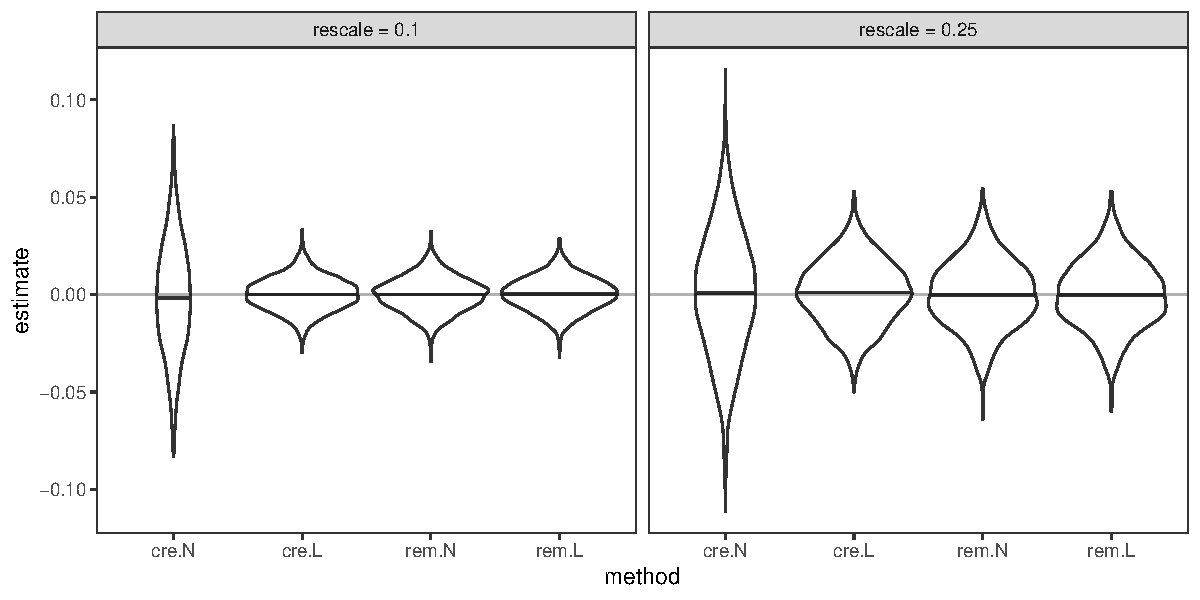
\includegraphics[width = \textwidth]{figures/RemReg_violin.pdf}
\caption{Simulation with $2000$ Monte Carlo replicates and $a=0.05$ for ReM} \label{fg::rerandomizationandancova}
\end{figure}


 


\section{Final remarks}

ReM uses the Mahalanobis distance as the balance criterion. We can consider general rerandomization with the balance criterion defined as a function of $\bm{Z}$ and $\bm{X}$.  For example, we can use the following criterion based on marginal tests for all coordinates of $X_i = (x_{i1}, \ldots, x_{iK})\tran$. We accept $\bm{Z}$ if and only if 
\begin{equation}
\label{eq::marginal-testing-rerandomization}
\left | \frac{  \hat{\tau}_{xk} }{   \sqrt{  \frac{n}{n_1 n_0} S_{xk}^2       }  }   \right | \leq  a \quad ( k=1,\ldots, K )
\end{equation}
for some predetermined constant $a > 0$, where $S_{xk}^2$ is the finite-population variance of covariate $x_{ik}$.  For example, $a$ is some upper quantile of a standard Normal distribution. See \citet{zhao2021no} for the theory for the rerandomization based on criterion \eqref{eq::marginal-testing-rerandomization} as well as other criteria. 


With a continuous outcome, Fisher's ANCOVA has been the standard approach for many years.  \citet{lin2013}'s improvement has better theoretical properties even when the linear model is misspecified. With a binary outcome, it is common to use the coefficient of the treatment in the logistic regression of the observed outcome on the intercept, the treatment indicator, and covariates to estimate the causal effects. However, \citet{freedman2008randomization} showed that this logistic regression does not have nice properties under the potential outcomes framework. Even if the logistic model is correct, the coefficient estimates the conditional odds ratio (see Chapter \ref{sec::logistic-regression}) which may not be the parameter of interest; when the logistic model is incorrect, it is even harder to interpret the coefficient. From the discussion above, if the parameter of interest is the average causal effect, we can still use \citet{lin2013}'s estimator to analyze the binary outcome data in the CRE. \cite{guo2020generalized} extend  \citet{lin2013}'s theory to allow for using generalized linear models to construct estimators for the average causal effect under the potential outcomes framework.  


Other extensions of \citet{lin2013}'s theory focus on high dimensional covariates. \citet{bloniarz2015lasso} focus on the regime with many covariates than the sample size, and suggest replacing the OLS fits with the least absolute shrinkage and selection operator (LASSO) fits \citep{tibshirani1996regression} of the outcome on the intercept, the treatment, covariates and their interactions. \citet{lei2018regression} focus on the regime with a diverging number of covariates without assuming sparsity, and under certain regularity conditions, they show that \citet{lin2013}'s estimator is still consistent and asymptotically Normal. \citet{wager2016high} propose to use machine learning methods to analyze high dimensional experimental data. 



\section{Homework Problems}

\paragraph{FRT under ReM}\label{hw::FRT-under-REM}

Describe the FRT under ReM.


\paragraph{Invariance of the Mahalanobis Distance}\label{para::invariance-M}

Prove Lemma \ref{lemma::invariance-mdistance}. 


\paragraph{Bias of the difference-in-means estimator under rerandomization}\label{hw::unbiasednessof-tauhat-rerandom}

Assume that we draw $\bm{Z} = (Z_1, \ldots, Z_n)$ from a CRE and accept it if and only if $\phi(\bm{Z}, \bm{X}) = 1$, where $\phi$ is a predetermined balance criterion. Show that if $n_1 = n_0$ and 
\begin{eqnarray}
\phi(\bm{Z}, \bm{X}) = \phi(\bm{1}_n-\bm{Z}, \bm{X}), \label{eq::symmetry}
\end{eqnarray}
then $\hat{\tau}$ is unbiased for $\tau$. 
Verify that rerandomization using the Mahalanobis distance satisfies \eqref{eq::symmetry} if $n_1 = n_0$. 
Give a counterexample that $\hat{\tau}$ is biased for $\tau$ when these two conditions do not hold.  


Remark: $\phi(\bm{Z}, \bm{X}) $ can be a general balance criterion in this problem. ReM is a special case with $\phi(\bm{Z}, \bm{X})  =  I(M\leq a) $.


\paragraph{Equivalent form of $R^2$ in the CRE}\label{para::r2-cre}

Prove Proposition \ref{prop::rsquared-forms}. 



\paragraph{More on linear projections of the potential outcomes onto covariates}\label{hw::projection-po-onto-x}



Show that
$$
S^2(1\mid X) = S_{Y(1)X} (S_X^2)^{-1} S_{XY(1)}
$$
where $S_{XY(1)}$ is the finite population covariance between $Y_i(1)$'s and $X_i$'s, $S_{Y(1)X} = S_{XY(1)}\tran$, and $S_X^2$ is the finite population covariance matrix of $X_i$'s. 
Find the analogous formulas for $S^2(0\mid X) $ and $S^2(\tau\mid X) .$



\paragraph{Comparing the true variances within the family of linearly adjusted estimator}\label{hw::compare-true-variance} 



Show that the variance $\hat{\tau}(\beta_1, \beta_0)$ decomposes into
$$
\var\{ \hat{\tau}(\beta_1, \beta_0) \} 
=  
\var\{ \hat{\tau}( \tilde{\beta}_1, \tilde{\beta}_0) \}  
+
\var\{ \hat{\tau}(\beta_1, \beta_0) - \hat{\tau}(\tilde{\beta}_1, \tilde{\beta}_0) \}
$$
where $\tilde{\beta}_1$ and $\tilde{\beta}_0$ are the coefficients of $X_i$ in the OLS projection of $Y_i(1)$'s and $Y_i(0)$'s onto $(1, X_i)$'s, respectively. 



Remark: \citet[][Example 9]{li2017general} derived the decomposition. It shows that based on the true variance, $\hat{\tau}( \tilde{\beta}_1, \tilde{\beta}_0)$ is an optimal choice within the family of linearly adjusted estimator because $\var\{ \hat{\tau}(\beta_1, \beta_0) - \hat{\tau}(\tilde{\beta}_1, \tilde{\beta}_0) \}$ is always non-negative.   




\paragraph{Lin's estimator for covariate adjustment}\label{para::lin-ols-covadj}

Prove Proposition \ref{prop::lin-ols}. 

\paragraph{Predictive and projective estimators}\label{para::predictiveestimator}
Prove \eqref{eq::predictiveestimator} and \eqref{eq::projectiveestimator}. 
 
 
 \paragraph{Equivalent form of the covariate-adjusted estimator}\label{para::reg-covariate-imbalance}

Prove \eqref{eq::linear-covariate-imbalance} and \eqref{eq::lin-covariate-imbalance}. 
 
 
 
\paragraph{ANCOVA also adjusts for covariate imbalance}
\label{para::ancova-imbalance}

This problem gives a result for ANCOVA that is similar to \eqref{eq::lin-covariate-imbalance}. 

Show that
$$
\hat{\tau}_\textsc{F} =\hat\tau  - \hat\gamma_\textsc{F}\tran \hat\tau_X,
$$
where $ \hat\gamma_\textsc{F}$ is the coefficient of $X_i$ in the OLS fit of $Y_i$ on $(1,Z_i, X_i)$. 





 \paragraph{Regression adjustment / post-stratification of CRE}\label{para::lin=ps-discrete}
 
 Prove Proposition \ref{prop::lin=ps-discrete}. 
 
 
Remark:  Sometimes $\hat{\tau}_{\textsc{ps}}$ or $ \hat{\tau}_\textsc{L}$ may not be well-defined. In those cases, we treat $\hat{\tau}_{\textsc{ps}}$ and $ \hat{\tau}_\textsc{L}$ as equal. You can ignore this complexity in the proof. 
 
%In a completely randomized experiment, we have a binary treatment indicator $Z$, an outcome $Y$, and a discrete covariate $X \in \{  1, \ldots, K \}$. We can use two methods to use covariates to improve estimation efficiency. 
%
%First, we can use the post-stratification estimator, pretending that the experiment is a stratified randomized experiment, conditional on $X$. This estimator is $\hat{\tau}_{\textsc{ps}}$. 
%
%Second, we can create $K-1$ dummy variables $\delta_{1i} = I(X_i=1), \ldots, \delta_{K-1,i} = I(X_i=K-1)$, and use Lin's estimator with covariates $\delta_1,\ldots, \delta_{K-1}$. This estimator is $\hat{\tau}_\textsc{L}$. 
%
%Show that $\hat{\tau}_{\textsc{ps}} = \hat{\tau}_\textsc{L}.$ Note that sometimes $\hat{\tau}_{\textsc{ps}}$ or $ \hat{\tau}_\textsc{L}$ may not be well-defined. In those cases, we treat $\hat{\tau}_{\textsc{ps}}$ and $ \hat{\tau}_\textsc{L}$ as equal. 


 
% \paragraph{Regression adjustment in the Fisher Randomization Test}
%This is a reanalysis of the LaLonde experimental data used in the lecture. In \texttt{FRTlalonde.R}, I conduct the Fisher randomization test using four test statistics. The Fisher randomization test can be more general with at least the following two additional strategies. Under the potential outcomes framework, {\it all potential outcomes and covariates are fixed numbers}. 
%
%
%First, we can use test statistics based on residuals from the linear regression. Run a linear regression of the outcomes on the covariates, and obtain the residuals (i.e., treat the residuals as the pseudo ``outcomes''). Then define the four test statistics based on the residuals. Conduct the Fisher randomization test using these four new test statistics. Report the corresponding $p$-values.
%
%
%Second, we can define the test statistic as the coefficient in the linear regression of the outcomes on the treatment and covariates. Conduct the Fisher randomization test using this test statistic. Report the corresponding $p$-value. 
%
%
%Why the five $p$-values from the above two strategies are exact $p$-values? Justify them. 


\paragraph{More on the difference-in-difference estimator in the CRE}\label{hw::did-CRE}

This problem gives more details for the difference-in-difference estimator in the CRE in Section \ref{sec::difference-in-difference-CRE}. 

Show that $\hat{\tau}(1,1) $ is unbiased for $\tau$, calculate its variance, and show that $\hat{V}( 1,1 ) $ is a conservative estimator for the true variance of $\hat{\tau}(1,1) $. When does $E\{\hat{V}( 1,1 ) \} = \var\{  \hat{\tau}(1,1)  \}$ hold?



Compare the variances of $\hat{\tau}(0,0) $ and $\hat{\tau}(1,1) $ to show that 
$$
\var\{ \hat{\tau}(0,0) \}  \geq \var\{  \hat{\tau}(1,1)  \}
$$
if and only if 
$$
2 \frac{n_0}{n} \beta_1 + 2\frac{n_1}{n} \beta_0 \geq 1,
$$
where 
$$
\beta_1 = \frac{\sum_{i=1}^n (X_i-\bar{X})\{  Y_i(1)-\bar{Y}(1) \}  }{  \sum_{i=1}^n (X_i-\bar{X})^2 },\quad
\beta_0 = \frac{\sum_{i=1}^n (X_i-\bar{X})\{  Y_i(0)-\bar{Y}(0) \}  }{  \sum_{i=1}^n (X_i-\bar{X})^2 }
$$
are the coefficients of $X_i$ in the OLS fits of $Y_i(1)$ and $Y_i(0)$ on $(1,X_i)$, respectively. 


Remark: \citet[][page 28]{gerber2012field} discussed a special case  of this problem with $n_1=n_0.$



\paragraph{Data re-analyses of the Penn Bonus Experiment}

 
Re-analyze the Penn Bonus Experiment data. The analysis in Chapter \ref{chapter::stratification-poststratification} uses the treatment indicator, the outcome, and the block indicator. Now we want to use all other covariates. 

Conduct regression adjustments within the strata of the experiment, and then combine these adjusted estimators to estimate the average causal effect. Report the point estimator, estimated standard error, and 95\% confidence interval. Compare them with those without regression adjustment. 
 

\paragraph{Missing outcomes in randomized experiments}\label{hw::missing-y-experiments}

The data analysis in Section \ref{sec::rem-reg-simulation} uses a naive imputation method to deal with missing outcomes. It is somewhat arbitrary. 

Impute the missing outcomes under the treatment and control, respectively,  based on the observed means. Do the results change?

Impute the missing outcomes under the treatment and control, respectively, based on linear regressions of the observed outcomes on the covariates. Do the results change? 

Do you have other ways to deal with missing outcomes? Justify them and implement them to analyze the dataset. 




\paragraph{Recommended reading}

The title of this chapter is the same as that of \citet{li2019rerandomization}, which studied the roles of rerandomization and regression adjustment in the design and analysis stages of randomized experiments, respectively. 


